\section{Auswertung}
\subsection{Vorbereitung}
Als Vorbereitung für den Verusch werden die Halbwertszeiten für $^{104}$Rh und $^{52}$V recherschiert. (Quellen: \cite{V} , \cite{Rh})
\begin{align}
    T_{^{52}\text{V}} = (224,5 \pm 0,3) \text{s}\\
    T_{^{104}\text{Rh}} = (42,3 \pm 0,4) \text{s}\\
    T_{^{104i}\text{Rh}} = (260,4 \pm 1,8) \text{s}\\
\end{align}
\subsection{Nullrate}
Über die aufgenommenen Daten für die Nullrate wurden diese Summiert und anschließend durch die Anzahl der Messwerte dividiert.
Der Mittlewert für die poissonverteilten Untergrundraten ergibt sich somit als:
\begin{align}
    N_{\text{U}} =  (139\pm 4) \; \frac{\text{Imp}}{300 \text{s}} \\
    \Delta N_{\text{U}} = \sqrt{ \sum_{i=1}^n \left( \frac{1}{n}\Delta N_{\text{U}_{\text{i}}} \right)^2}
\end{align}
Mit der Anzahl $n$ der Messwerte. In diesem Experiment gilt $n = 7$.
\subsection{Vanadium}
Um mit den Berechnungen zu Beginnen muss zunächst die Untergrundrate von den messwerten abgezogen werden.
Da die Messung der Impulsrate von Vanadium in 30 Sekunden Intervallen gemacht wurde wird $N_{\text{U}}$ auf das passende Intervall angepasst.
\begin{align*}
    N_{\text{U},\text{Vanadium}} =  \frac{N_{\text{U}}}{10} = (13,9 \pm 0,4) \; \frac{\text{Imp}}{30\text{s}}
\end{align*}
\begin{figure}
    \centering
    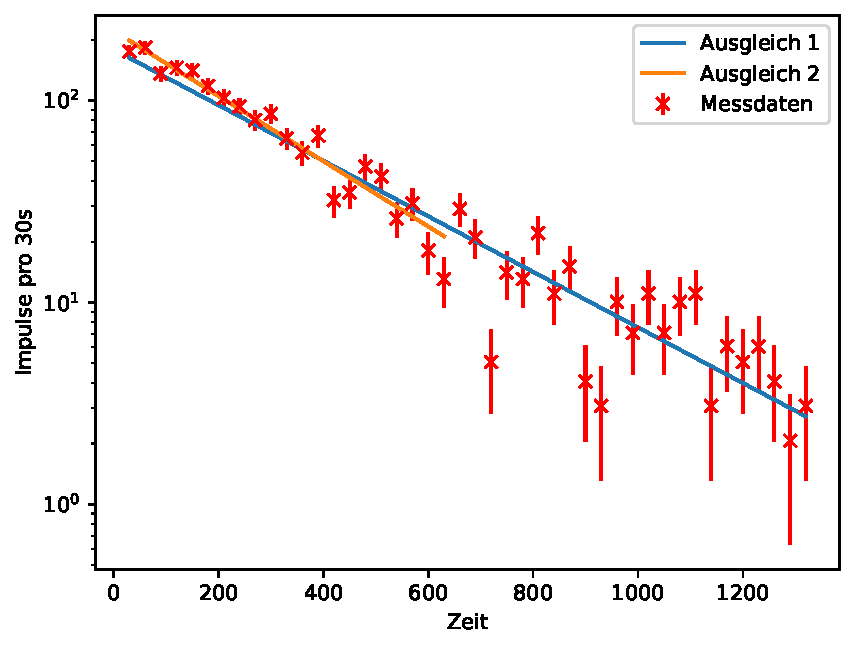
\includegraphics[width=0.7\textwidth]{plots/Vanadium.pdf}
    \caption{Darstellung der Impulse pro 15s zum Zeitpunkt $t$ in einem halblogarithmischen Plot.\\
    Zur Bestimmung der Zerfallsrate wird zunächst das gesamte Zahlrratenintervall verwendet. 
    Aufgrund der geringen Zählrate am Ende des Intervalls, welche in den Untergrund eingeht, wird eine
    weitere Ausgleichsgerade gezogen, für welche das Intervall bis zur doppelten Halbwertszeit gewählt wird. }
\end{figure}
Mit \ref{eqn:Zerfallsgesetz} wird nun ein linearer Ausgleich gefertigt. \\
Für den blauen ''Ausgleich 1'' ergibt sich:
\begin{align*}
    \ln(N(t)) = m \cdot t + b\\
     m = (-0,00317 \pm 0,00016)\si{s^{-1}} && b = (5,19 \pm 0,13) \\
    \lambda = -m = (0,00317 \pm 0,00016)\si{s^{-1}} \\
    T1_{^{52}\text{V}} = \ln\left( \frac{2}{\lambda} \right) = (219 \pm 11) \si{s}
\end{align*}
Und für den orangenen ''Ausgleich 2'' mit gleicher Funktion:
\begin{align*}
     m = (-0,00372 \pm 0,00023)\si{s^{-1}} && b = (5,40 \pm 0,08) \\
    \lambda = -m = (0,00372 \pm 0,00023)\si{s^{-1}} \\
    T2_{^{52}\text{V}} = \ln\left( \frac{2}{\lambda} \right) = (186 \pm 11) \text{s}
\end{align*}

\subsection{Rhodium}
Auch für die Messwerte des Rhodium zerfalls muss die Nullrate herausgerechnet werden.
Dazu wird selbige wieder an das Intervall, in diesem Fall 15 Sekunden, angepasst.
\begin{align*}
    N_{\text{U},\text{Rhodium}} =  \frac{N_{\text{U}}}{20} = (6,96 \pm 0,22) \; \frac{\text{Imp}}{30\text{s}}
\end{align*}
\begin{figure}
    \centering
    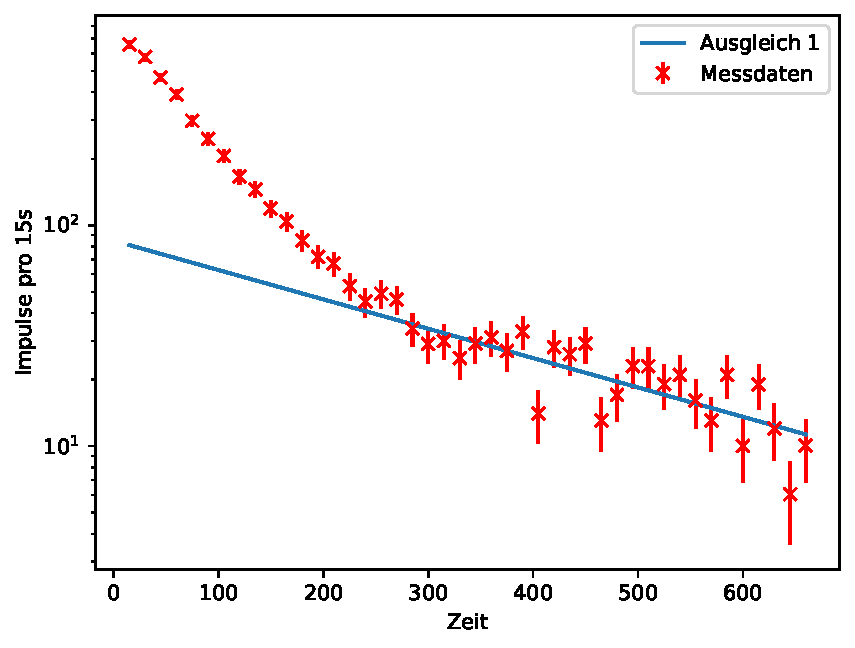
\includegraphics[width=0.7\textwidth]{plots/Rhodium_lang.pdf}
    \caption{Die Impuls pro $15$s zum Zeitpunkt $t$ halblogarithmisch dargestellt.\\
    Es werden zwei Teilbereiche deutlich, die auf die Teilreaktionen \ref{eqn:rh} zuückzuführen sind.
    Dabei wird der kurzlebige Zerfall vom langlebigen Zerfall überlagert.\\
    Die Ausgleichsgerade wird hierbei nur für den langlebigen Zerfall betrachtet.}
    \label{fig:langlebigRH}
\end{figure}
Aus dem Ausgleich ergibt sich für den langsamen Zerfall:
\begin{align*}
    \ln(N(t)) = m \cdot t + b\\
     m = (-0,0031 \pm 0,0006)\si{s^{-1}} && b = (4,44 \pm 0,31) \\
    \lambda = -m = (0,0031 \pm 0,0006)\si{s^{-1}} \\
    T_{^{104i}\text{Rh}} = \ln\left( \frac{2}{\lambda} \right) =  (230 \pm 50) \text{s}
\end{align*}
Um eine Aussage über die Halbwertszeit $T$ des kurzlebigen Zerfalls, welcher vom langlebigen Zerfall
überlager wird, zu machen, muss zunächst der Zählratenanteil $N_{\text{langl.}}(t)$ abgezogen werden.
Über eine Regression am langlebigen Anteil aus Abb. \ref{fig:langlebigRH} kann somit
auf die Zählrate des kurzlebigen Zerfalls zurückgeschlossen werden.
Es ergibt sich
\begin{align}
    N_{\text{kurzl.}}&=N_{\text{gesamt}}-N_{\text{langl.}}.
\end{align} 
Für $N_{\text{langl.}}$ ergibt sich über die Regression
\begin{align}
   N _{\text{langl.}}=e^{m \cdot t +b}.
\end{align}
Somit folgt für die Impulsrate $N$ zum Zeiptunkt $t$ für den kurzlebigen Zerfall
\begin{figure}
    \centering
    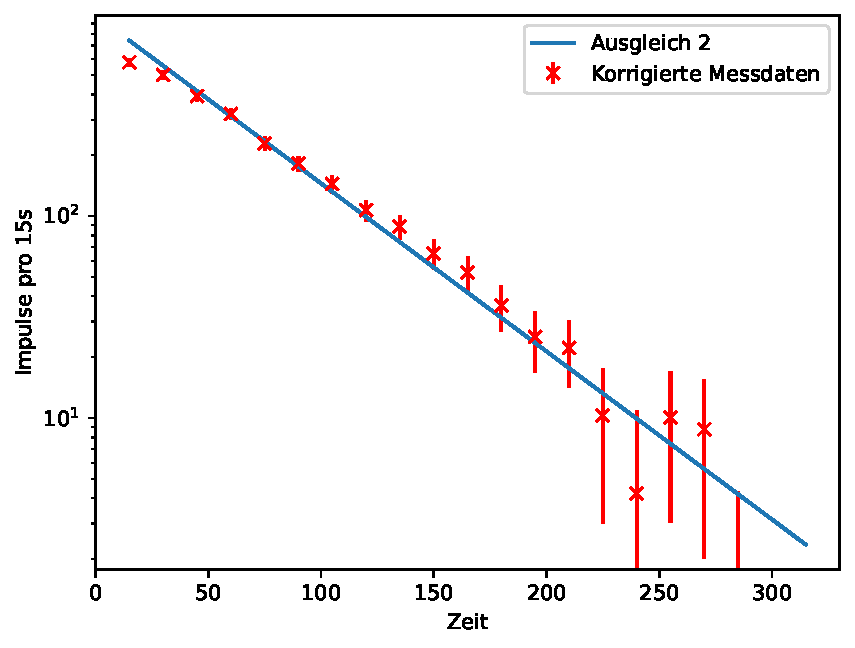
\includegraphics[width=0.7\textwidth]{plots/Rhodium_kurz.pdf}
    \caption{Die Impulse pro $15$s zum Zeitpunkt $t$ für den kurzlebigen Zerfall halblogarithmisch aufgetragen.}
\end{figure}
\begin{align*}
     m = (-0,0192 \pm 0,0009)\si{s^{-1}} && b = (6,89 \pm 0,14) \\
    \lambda = -m = (0,0192 \pm 0,0009)\si{s^{-1}} \\
    T_{^{104}\text{Rh}} = \ln\left( \frac{2}{\lambda} \right) = (36,2 \pm 1,7) \text{s}
\end{align*}
